\chapter{Background}
\label{chapter:background}
\section{Call and Put Options}
As stated before, call and put options enable their buyer to respectively buy and sell the underlying stock at the maturity for the fixed strike price.
In the case of a call option, if at the maturity the market price of its underlying asset is greater than the strike, investors can exercise the option and buy the asset for the fixed strike price. Then they can immediately go to the market and sell the asset for its higher value. Thus, in this case, the payoff of the option would be the difference between these two prices. On the other hand, if at the maturity the price of the asset decreases past the strike, the investor should let the option expire, since the asset is available in the market for a price lower than the strike. In this case, the payoff of the option would be zero.
The same reasoning can be made for put type options.
The payoff function of these two types of options can then simply be deduced as
\begin{equation}\label{callput}
\begin{split}
&\text{Payoff}_\text{call}=\max\left(S(T)-K,0\right);\\
&\text{Payoff}_\text{put}=\max\left(K-S(T),0\right),
\end{split}
\end{equation}
\noindent where $K$ is the strike price and $S(T)$ is the asset price, $S(t)$, at the maturity, $T$. These functions are represented in \autoref{fig:Payoff}.

\begin{figure}[!htb]
    \centering
      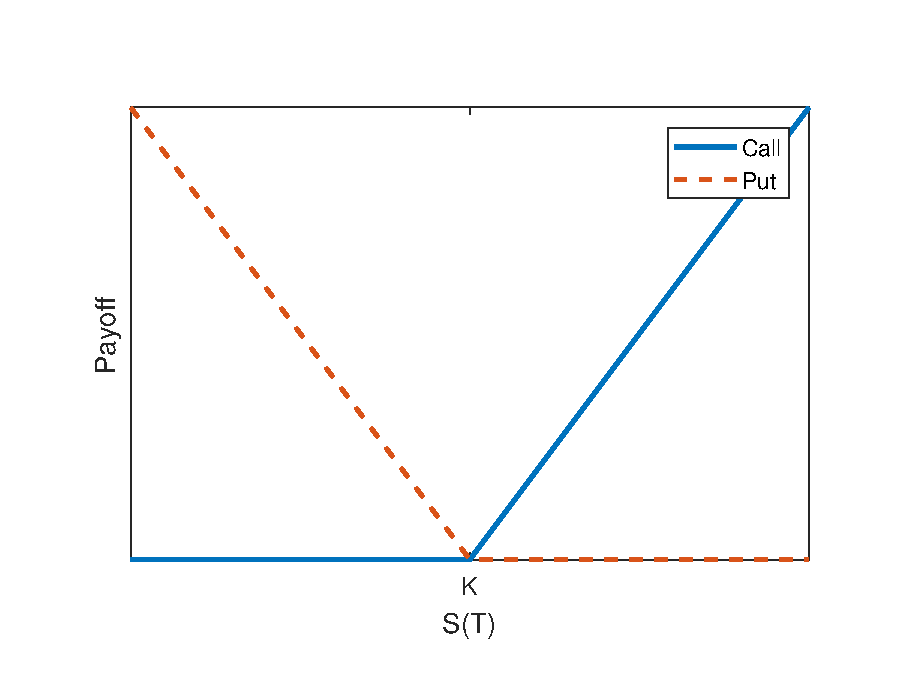
\includegraphics[width=.5\columnwidth]{Payoff.eps}
      \caption[Payoff functions of call and put options]{Payoff functions of \emph{call} and \emph{put options}.}\label{fig:Payoff}
    \end{figure}
    
With eqs.\eqref{callput} in mind, it should be clear that the value of these two types of options corresponds to their expected future payoff discounted back to the present, which gives
\begin{equation}
\begin{split}
&C(K,T)=e^{-rT}\mathbb{E}\left[\max\left(S(T)-K,0\right)\right]=e^{-rT}\mathbb{E}\left[\left(S(T)-K\right)\mathbbm{1}_{\left\{S(T)>K\right\}}\right];\\
&P(K,T)=e^{-rT}\mathbb{E}\left[\max\left(K-S(T),0\right)\right]=e^{-rT}\mathbb{E}\left[\left(K-S(T)\right)\mathbbm{1}_{\left\{S(T)<K\right\}}\right],
\end{split}
\end{equation}
\noindent with $C(K,T)$ and $P(K,T)$ being the values of call and put options, respectively. $\mathbb{E}[\cdot]$ and $\mathbbm{1}_{\{\cdot\}}$ correspond to the expected value and indicator functions, respectively.




    
\section{Black-Scholes-Merton Formulae}
\label{section:Black-Scholes-Merton Formulae}
Due to their high importance, options have been studied in great detail in the past.
Probably the most important result in this field came from Fischer Black, Myron Scholes and Robert Merton, who developed a mathematical model to price options - the famous Black-Scholes-Merton model~\cite{Scholes} - still in use in present days~\cite{Wilmott3}.

This model states that the price of an European call or put option, whose underlying asset is a stock, follows the partial differential equation (PDE)

\begin{equation}\label{BS2}
\pdv{V}{t}+\frac{1}{2}\sigma^2S^2\pdv{^2V}{S^2}+rS\pdv{V}{S}-rV=0,
\end{equation}

\noindent where $V$ is the price of the option, $S$ is the price of the underlying stock, $r$ is the risk-free interest rate and $\sigma$ is the stock price volatility.

\hl{underlying asset=stocks}
 
The risk-free interest rate, $r$, is the interest an investor would receive from any risk-free investment (e.g. treasury bills). An investor should never invest in risky products whose expected return is lower than this interest, since there's the alternative of obtaining a higher payoff without the disadvantage of taking risks. In general, this rate changes slightly with time and is unknown, but Black \textit{et al.}, in their original model (eq.\eqref{BS2}), assumed that it remains constant throughout the option's duration and that it is known. Some later developments dealt with this shortcoming, providing models to replicate the behavior of interest rates~\cite{HJM}, but because option prices do not significantly depend on this value~\cite{Wilmott3}, in the remainder of this thesis we shall assume it is constant and known.

Finally, the volatility, $\sigma$, is a measure of uncertainty and will be studied in more detail in section \ref{section:volatility}.

One important assumption of the Black-Scholes-Merton model is that stock prices follow a stochastic process, known as Geometric Brownian Motion (GBM), which can be defined as
\begin{equation}\label{GBM}
dS(t)=rS(t)dt+\sigma S(t)dW(t),
\end{equation}
\noindent with $\{W(t),\ t>0\}$ defining a one-dimensional Brownian motion.


With this result, pricing options is fairly straightforward - we simply need to solve the PDE in eq.\eqref{BS2} in a similar fashion to the initial value problem for the diffusion equation~\cite{Dilao}.
The results published in the original article by Black \textit{et al.} state that, at time $t$, call and put options can be valued as
\begin{equation}\label{callputBS}
\begin{split}
&C(S(t),t)=N(d_1)S(t)-N(d_2)Ke^{-r(T-t)};\\
&P(S(t),t)=-N(-d_1)S(t)+N(-d_2)Ke^{-r(T-t)},
\end{split}
\end{equation}
\noindent where $N(\cdot)$ is the cumulative distribution function of the standard normal distribution and $d_1$, $d_2$ are given by
\begin{equation}\label{d1d2}
\begin{split}
&d_1=\frac{1}{\sigma\sqrt{T-t}}\left[\ln\left(\frac{S_t}{K}\right)+\left(r+\frac{\sigma^2}{2}\right)(T - t)\right];\\
&d_2=d_1-\sigma\sqrt{T-t}.\\
\end{split}
\end{equation}



From eq.\eqref{callputBS} we can derive the relationship between $C(S,t)$ and $P(S,t)$, known as the \emph{put-call parity}
\begin{equation}
C(S(t),t)=S(t)-Ke^{-r(T-t)}+P(S(t),t).
\end{equation}
\noindent Because of this duality, we can always obtain the prices of put options from the prices of call options with the same underlying asset, maturity and strike. For this reason, providing results for both option types is redundant and unless otherwise stated, all options will be assumed European calls in the following sections.


\section{Volatility}
\label{section:volatility}
Volatility is a measure of the uncertainty of future stock price movements. In other words, a high volatility will lead to great future fluctuations in the stock price, whereas a stock with low volatility is more stable.

\hl{put image of varying volatilities here}

Of all the parameters in the Black-Scholes formula (eq.\eqref{BS2}), volatility is the only one we can't easily measure from market data.
Furthermore, unlike the interest rate, volatility has a great impact on the behavior of stock prices and consequently on the price of options~\cite{Wilmott3}.
These two factors make volatility one of the most important subjects in all of mathematical finance and thus the focus of much research.



It should be noted that there are several types of volatility, depending on what is being measured. Some of these types will be approached in the next subsections.

\subsection{Implied Volatility}
\label{section:impliedvolatility}
\emph{Implied volatility} can be described as the value of stock price volatility that, when input into the Black-Scholes pricer in eq.\eqref{callputBS}, outputs a value equal to the market price of a given option.
In other words, it would be the stock price volatility that the seller/buyer of the option assumed when pricing it (given that the Black-Scholes model was used).

Because eq.\eqref{callputBS} is not invertible, we need to use some numerical method (e.g. Newton's method) to find the value of implied volatility that matches the market and model prices. In other words, we must find numerically the solution to the equation
\begin{equation}\label{impvolform}
C(\sigma_{imp},S(t),t)-\overline{C}=0,
\end{equation}
\noindent where $C(\sigma_{imp},\cdot)$ corresponds to the result of eq.\eqref{callputBS} using the implied volatility $\sigma_{imp}$ and $\overline{C}$ is the price of the option observed in the market.

We can obtain the implied volatility of an option from its price and vice versa, because eq.\eqref{callputBS} is monotonic in the volatility. This duality is so fundamental that investors often disclose their options by providing their implied volatility instead of their price~\cite{Wilmott}.

One interesting property of implied volatility is that, in the real-world, it depends on the strike price and the maturity. In the Black-Scholes world this should not occur. If investors really used the this model to price their options, two options with the same underlying asset should have the same implied volatility, regardless of their strike prices or maturities (i.e. the same underlying asset doesn't have two different volatilities at the same time).
However, when observing real market data, this is indeed what is observed.

The implied volatilities' dependence on the strike price is a function that can take one of two forms, known as \emph{smile} and \emph{skew}.
An implied volatility smile shows greater values of $\sigma_{imp}$ for options with strikes farther from the current stock price. The minimum occurs where the strike equals the current stock price. A skew, on the other hand, only shows greater $\sigma_{imp}$ in one of the directions (i.e. for strikes either bigger or smaller than the current stock price). Both phenomena are represented in \autoref{fig:smileskew}.

Because of their higher implied volatility, we can conclude that options with strikes different from the current stock price are overpriced.
The reason behind this odd market behavior is related to the simple demand-supply rule~\cite{Wilmott3}. On the one hand, some investors are risk-averse and want to hedge their losses in case of a market crash (as explained in subsection \ref{subsection:why options are important}). They don't mind paying a higher price for an option if this means they would be relatively safe from potentially devastating market crashes. For this reason, the prices of (call) options with lower strikes increase, driving their implied volatility up. On the other hand, other investors are risk-seekers and want to take advantage of possible sudden price increases, buying the stocks for the lower strike prices. They don't mind paying higher prices for the options and this drives the prices of high strike options (and, consequently, their implied volatility) up. This fear-greed duality gives rise to the observed volatility smile.
   
    
\begin{figure}[!htb]
  \begin{subfigmatrix}{2}
    \subfigure[Smile]{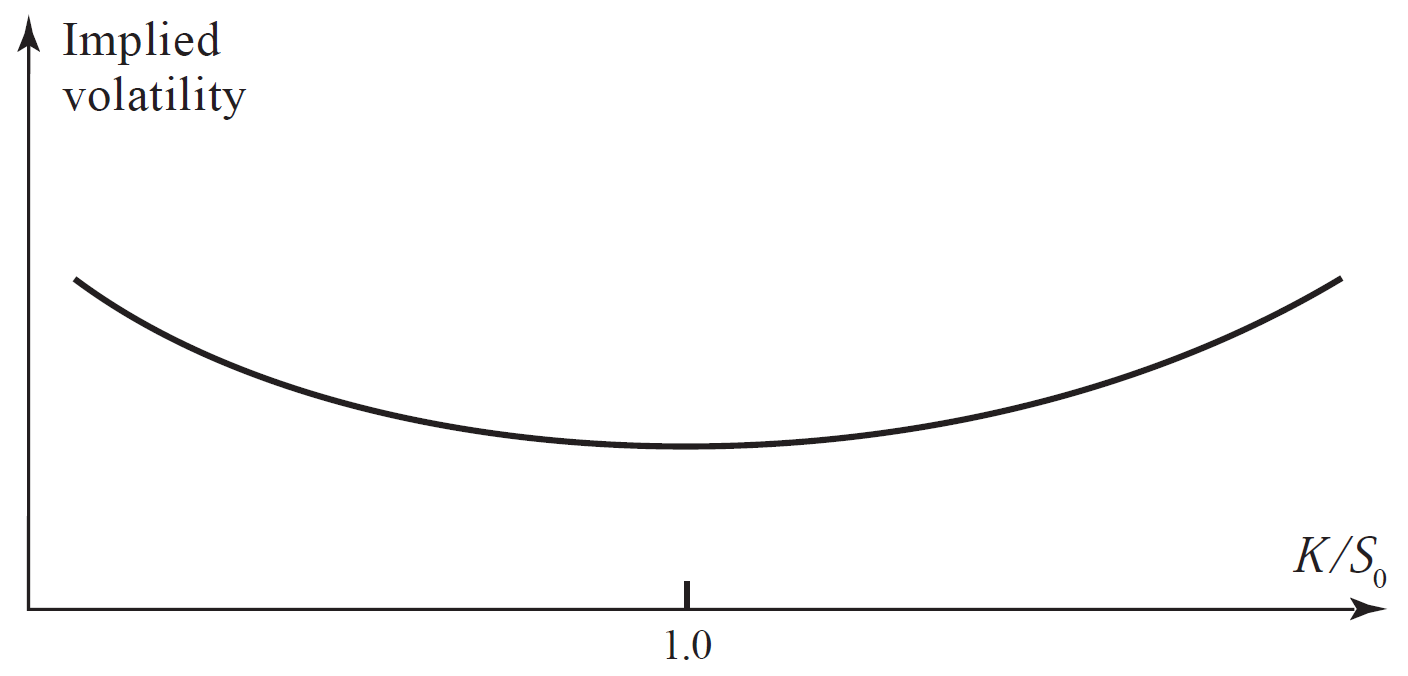
\includegraphics[height=0.20\linewidth]{Smile.png}}
    \subfigure[Skew]{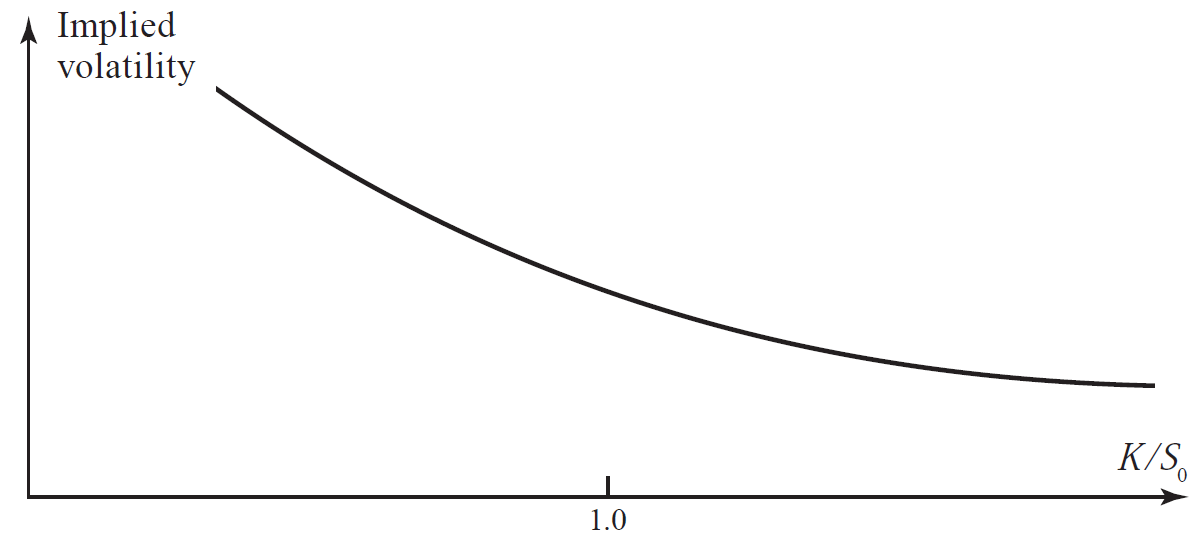
\includegraphics[height=0.20\linewidth]{Skew.png}}
  \end{subfigmatrix}
  \caption[Example of an implied volatility smile (left) and skew (right).]{Example of an implied volatility smile and skew.\hl{source=Hull}}
  \label{fig:smileskew}
\end{figure}

The dependence of the implied volatility on the maturity date is more complex, but in general it decreases with $T$.

It can also be shown that the implied volatility is the same for calls and puts~\cite{Hull}.

\subsection{Local Volatility}
\label{subsection:localvolatility}
In their original work, Black \textit{et al.} assumed that volatility is constant throughout the whole contract. From market data, it can be clearly seen that this is not the case. There may be times where new information reaches the market and trading increases, driving volatility up. On the other hand, if investors are waiting for some new information to reach the market (e.g. the results of an election) trading may stall, and volatilities go down. 

The model in eq.\eqref{callputBS} is therefore not enough to completely grasp real-world trading. We should have a model where volatility is dynamic, measuring the uncertainty on the stock price at any point in time.
However, as we saw in subsection \ref{section:impliedvolatility} for implied volatility, the market's view of volatility also changes with the strike price. A volatility model that merely depends on time is thus insufficient.

The volatility should therefore be a function of both time and strike price: $\sigma(K,t)$. We call this model \emph{local volatility} and the geometric Brownian motion from eq. \ref{GBM} is transformed into
\begin{equation}\label{GBM2}
dS(t)=rS(t)dt+\sigma(K,t)S(t)dW(t),
\end{equation}
\noindent where $\sigma(K,t)$ is some function of $K$ and $t$.


Finding the local volatility function is not very important when pricing typical European options, because we can simply find the implied volatility from similar options in the market and assume a constant volatility throughout the option's duration.
However, for other contracts, such as American, Asian or Barrier options (among others) where the option's value depends on the intermediate stock prices, this function is indeed very useful.

Because we can't directly measure the local volatility of a stock from market data, we need some models to find it. The best known of these is Dupire's formula.

\subsubsection{Dupire's Formula}
\label{subsubsection:Dupire}
\hl{notation problems... T=T', K=K'}
One of the most famous results in the modelling of the local volatility function was obtained by Dupire~\cite{Dupire}. In his article, the author derives a theoretical formula for $\sigma(K,t)$, given by
\begin{equation}\label{dupire}
\sigma(K,T)=\sqrt{\frac{\displaystyle\pdv{C}{T}+rK\pdv{C}{K}}{\displaystyle\frac{1}{2}K^2\pdv{^2C}{K^2}}},
\end{equation}
\noindent where $\sigma(S,t)$ is the local volatility function for stock prices $S$ at time $t$ and $C=C(K,T)$ is the price of an European call option with strike price $K$ and maturity $T$.
A brief demonstration of this formula can be found in Appendix \ref{chapter:dupireformuladerivation}.


As can be seen, we need to differentiate the option prices with respect to their strikes and maturities. To achieve this, we need to gather from the market a large number of prices for options with different maturities and strikes, and perform some interpolation on them to obtain an option price surface (with $K$ and $T$ as variables). We then calculate the gradients of this interpolated surface and input them into eq. \ref{dupire} to obtain the local volatility surface.

Even before implementation, four potential sources of error can be found:
\begin{itemize}
\item First, it should be noted that markets only trade options with very specific maturities (e.g. 1, 2, 4 and 6-months maturity). For this reason, our data will be very sparse with respect to maturity and the interpolation obtained may not perform as required.
\item Furthermore, it can be shown that, for options with strikes very different from the current stock price, the option's price is approximately linear with respect to the strike. The second derivative in these regions would therefore be very close or even equal to zero. Because this second derivative is in the denominator of eq.\eqref{dupire}, our volatilities may explode for very large or very small strikes.
\item There is also the problem of noise. Because we are interpolating very sparse data, even small fluctuations in the option market price will cause variations in the option price interpolation. This can be very problematic in regions where the second derivative is small, because the result is very sensitive to this value.
\item Finally, some problems arise from the market itself. While most investors use some theoretical basis in their trades, the market is still governed by the demand-supply rule. If too many investors want to buy the option and few want to sell it, the option price will increase, even if it means that the option will be overpriced, and vice versa. It may also happen that the market is not liquid enough (i.e. very few trades or even no trades at all occur for some options with very large maturities or very large/small strikes or for some options on relatively unknown stocks) causing the option prices to not truly follow the market's perception of future price movements.
\end{itemize}
All these problems must be taken into account when applying Dupire's model.

Besides, it can be shown that if the local volatility surface truly matched reality, it should remain unchanged (i.e. the local volatility surface measured today and in one month's time should, in theory, be the same). However, by studying market data, we can see that this is really not the case~\cite{Wilmott3}. We can therefore conclude that the model doesn't completely correspond to reality and for that reason it shouldn't be used blindly.


Some authors have also pointed out that the volatility smile obtained from Dupire's local-volatility model doesn't follow real market dynamics~\cite{Hagan}. They demonstrate that when the price of the stock either increases or decreases, the volatility smile predicted by the model shifts in the opposite direction. The minimum of the volatility smile would therefore be offset and no longer correspond to the local stock price. The volatility smile dynamics obtained from the local-volatility model would then be actually even worse than if we assumed a constant volatility.


Dupire also developed an alternative local-volatility formula based on the implied volatility surface rather than the option price's, as seen in eq.\ref{dupire}.
The relation obtained is as follows
\begin{equation}\label{dupire2}
\sigma(K,T)=\sqrt{\frac{\displaystyle\sigma_{imp}^2+2(T-t)\sigma_{imp}\pdv{\sigma_{imp}}{T}+2rK(T-t)\sigma_{imp}\pdv{\sigma_{imp}}{K}}{\displaystyle\left(1+Kd_1\sqrt{T-t}\pdv{\sigma_{imp}}{K}\right)^2+K^2(T-t)\sigma_{imp}\left(\pdv{^2\sigma_{imp}}{K^2}-d_1\left(\pdv{\sigma_{imp}}{K}\right)^2\sqrt{T-t}\right)}},
\end{equation}
\noindent where $d_1$ is given by
\begin{equation}
d_1=\frac{\log(S(t)/K)+\left(r+\frac{1}{2}\sigma_{imp}^2\right)(T-t)}{\sigma_{imp}\sqrt{T-t}},
\end{equation}
\noindent with $t$ representing the current time (usually $t=0$), $T$ being the time at which the local volatility is being measured, and $S(t)$ the stock price at time $t$. We assume that $\sigma_{imp}=\sigma_{imp}(K,T)$ is the interpolated surface of the implied volatilities evaluated at time $T$, and price $K$.
This relation might be more useful than eq.\eqref{dupire} because the interpolated implied volatility surface \hl{might be smoother than the option price's}. We will compare the results from both formulas in the next chapters.




Despite all of its shortcomings, Dupire's formula is nonetheless very much used by traders to find the local volatility surfaces of assets and with them price exotic options afterwards.

\subsection{Stochastic Volatility}
\label{subsection:stochastic volatility}
As stated before, the volatility is not constant, is not observable and is not predictable, despite our attempts to model it. This seems to indicate that volatility is itself a stochastic process. Some research has been done into this hypothesis, and many models have been developed to replicate real-world volatilities.

As before, we assume that the stock price follows a geometric Brownian motion
\begin{equation}\label{stochvol}
dS(t)=rS(t)dt+\sigma(t)S(t)dW_1(t),
\end{equation}
\noindent but we further hypothesize that the volatility follows
\begin{equation}
d\sigma(t)=p(S,\sigma,t)dt+q(S,\sigma,t)dW_2(t),
\end{equation}
\noindent where $p(S,\sigma,t)$ and $q(S,\sigma,t)$ are some functions of the stock price $S$, time $t$ and of the volatility $\sigma$ itself. We also assume that $W_1$ and $W_2$ are two Brownian motion processes with a correlation of $\rho$, which gives
\begin{equation}
dW_1dW_2=\rho dt.
\end{equation}
\noindent This correlation factor $\rho$ can be explained by the relationship between prices and volatilities. Usually, when prices decrease, trade goes up and with it, rises the volatility. The inverse is true when prices increase. This seems to indicate a negative correlation between stock prices and volatilities, but positive correlations are also possible.

\iffalse
\hl{This correlation can be explained by the relationship between prices and volatilities.} As an example, we can consider a stock that costs \textdollar100 and changes by \textdollar0.10 daily. We can estimate, even without calculations, that it is very stable and thus has a low volatility.
On the other hand if another stock costs \textdollar1 and changes by \textdollar0.10 in a day, we can see that it is extremely volatile even though it changed by the same amount as the first. With this example, we can see that the volatility has some correlation with the stock price.
\fi

Choosing the right functions $p(S,\sigma,t)$ and $q(S,\sigma,t)$ is very important since the whole evolution of the stock price depends on them. All stochastic volatility models present a different version of these functions, and each may be more adequate for some types of assets. Furthermore, these functions have some parameters that we have to calibrate in order to best fit our model to market data.

We now present two of the most used stochastic volatility models - \emph{Heston} and \emph{SABR}.



\subsubsection{Heston Model}
One of the most popular stochastic volatility models is known as \emph{Heston model}. It was developed in 1993 by Steven Heston~\cite{Heston} and it states that our stock prices satisfy the relations
\begin{equation}
dS=\mu Sdt+\sqrt{\nu}SdW_1,
\end{equation}
\begin{equation}
d\nu=\kappa(\overline{\nu}-\nu)dt+\chi\sqrt{\nu}dW_2,
\end{equation}
\noindent with $\nu$ corresponding to the variance (i.e. $\nu=\sigma^2$) and where $W_1$ and $W_2$ have a correlation of $\rho$. \hl{Note that our stock price is now governed by a drift parameter $\mu$, unlike the usual risk-free measure drift of $r$, as seen in eq.} \eqref{GBM}. \hl{A transformation into the risk-free measure, using Gisarnov's theorem, is possible but the original model used the drift parameter $\mu$.}
The parameters $\kappa$, $\overline{\nu}$ and $\chi$ are, respectively, the mean-reversion rate (i.e. how fast the volatility converges to its mean value), the long-term variance (i.e. the mean value of variance) and the volatility of volatility (i.e. how erratic is the volatility evolution).

\hl{Feller condition}

One of the main advantages that make the Heston model so popular is that there is a closed-form solution for the prices of options priced under this model, which is given by
\begin{equation}\label{CH}
\begin{split}
C_{H}(\theta;K,T)&=e^{-rT}\mathbb{E}\left[\left(S(T)-K\right)\mathbbm{1}_{\left\{S(T)>K\right\}}\right]\\
&=e^{-rT}\left(\mathbb{E}\left[S(T)\mathbbm{1}_{\left\{S(T)>K\right\}}\right]-K\mathbb{E}\left[\mathbbm{1}_{\left\{S(T)>K\right\}}\right]\right)\\
&=S(0)P_1-e^{-rT}KP_2,
\end{split}
\end{equation}
\noindent where $C_{H}(\theta;K,T)$ corresponds to the theoretical European call option price under the Heston model, assuming a set of parameters $\theta$, strike K and maturity T. The variables $P_1$ and $P_2$ are given by
\begin{equation}\label{P1}
P_1=\frac{1}{2}+\frac{1}{\pi}\int_0^\infty\operatorname{Re}\left(\frac{e^{-iu\log K}}{iuf}\phi(\theta;u-i,T)\right)du,
\end{equation}
\begin{equation}\label{P2}
P_2=\frac{1}{2}+\frac{1}{\pi}\int_0^\infty\operatorname{Re}\left(\frac{e^{-iu\log K}}{iu}\phi(\theta;u,T)\right)du,
\end{equation}
\noindent where $i$ is the imaginary unit, $f$ is the forward price (i.e. $f=S(0)e^{rT}$) and $\phi(\theta;u,t)$ is the characteristic function of the logarithm of the stock price process. The characteristic function of a random variable is the Fourier transform of the probability density function of that variable.

Now we just have to find the appropriate characteristic function $\phi(\theta;u,t)$ in order to evaluate the integrals in eqs.\eqref{P1} and \eqref{P2} and find the option price with eq.\eqref{CH}. In the original article, Heston derived this very characteristic function~\cite{Heston} but it presented some discontinuities for large maturities and wasn't easily derivable. These shortcomings led some other authors to propose several modified versions of this function. Most recently, Cui \textit{et al.}~\citep{Cui} presented a characteristic function that not only doesn't have the previously mentioned discontinuities but is also easily derivable, given by
\begin{equation}
\phi(\theta;u,t)=\exp\left\{iu\left(\log S_0+rt\right)-\frac{t\kappa\overline{\nu}\rho iu}{\chi}-\nu_0A+\frac{2\kappa\overline{\nu}}{\chi^2}D\right\},
\end{equation}
\noindent with $A$ and $D$ given by
\begin{equation}
A=\frac{A_1}{A_2},
\end{equation}
\begin{equation}
D=\log d+\frac{\kappa t}{2}-\log A_2,
\end{equation}
\noindent where we introduce the variables $A_1$, $A_2$, $d$  and $\xi$
\begin{equation}
A_1=(u^2+iu)\sinh\frac{dt}{2},
\end{equation}
\begin{equation}
A_2=e^{dt/2}\left(\frac{d+\xi}{2}+\frac{d-\xi}{2}e^{-dt}\right),
\end{equation}
\begin{equation}
d=\sqrt{\xi^2+\chi^2(u^2+iu)},
\end{equation}
\begin{equation}
\xi=\kappa-\chi\rho iu.
\end{equation}

With this result, the calibration of the Heston model can be easily processed. We simply have to find the model parameters $\theta$ that minimize the difference between the model generated option prices, $C_H(\theta;K,T)$, and the market prices, $\overline{C}$. This calibration will be explored in detail in the next sections.

\iffalse
Calibrating the parameters  $\rho$, $\kappa$, $\overline{\nu}$ and $\chi$ is absolutely critical. A model with badly calibrated parameters would output wrong predictions, rendering it completely useless.
This calibration requires a fair amount of past market data and is by far the most complex and computationally demanding section of this model. We will deal with it in the next section.
\fi





\subsubsection{SABR Model}
One other very famous model for stochastic volatility was developed by Hagan \textit{et al.}~\cite{Hagan} and is known as \emph{SABR}. It stands for "\emph{stochastic-}$\alpha\beta\rho$" and in this model it is assumed that the option prices and volatilities follow
\begin{equation}\label{dF}
dF=\sigma F^\beta dW_1,
\end{equation}
\begin{equation}\label{dsigma}
d\sigma=\nu\sigma dW_2,
\end{equation}
\noindent with $F$ being the forward price (related to the spot price $S$ by $F(t)=S(t)e^{r(T-t)}$).
We further define $\alpha=\sigma(0)$ as the starting volatility, $f=F(0)=S_0e^{rT}$ as the starting forward price. Finally, as before, the two Brownian motion processes $W_1$ and $W_2$ have a correlation of $\rho$.

\iffalse
It should be noted that we are now using the \hl{forward measure}, so in eq.\eqref{dF} we use $F$, the \emph{forward price}, instead of the usual spot price $S$ from eq.  \ref{GBM}. These two quantities are related by $S(t)=e^{-r(T-t)}F(t)$, so we can easily obtain one from the other.
\fi


In the original article, the authors claim that $\beta$ can be fitted from historical market data, but usually investors choose this value arbitrarily, depending on the type of assets traded. Typical values used are $\beta=1$ (stochastic lognormal model), usually for foreign exchange options, $\beta=0$ (stochastic normal model), typical for interest rate options where forwards $f$ can be negative, and $\beta=0.5$ (stochastic CIR model), also common for interest rate options.

One of the main reasons why SABR is so popular is due to the quasi-closed-form solutions that greatly simplify its calibration. With the corrections done by Oblój~\cite{Obloj} on Hagan's original formula, it can be shown that the implied volatilities of options priced under the SABR model are given by
\begin{equation}
\begin{split}
\sigma_{SABR}(K,f,T)\approx&\frac{1}{\displaystyle\left[1+\frac{(1-\beta)^2}{24}\log^2\left(\frac{f}{K}\right)+\frac{(1-\beta)^4}{1920}\log^4\left(\frac{f}{K}\right)\right]}.\left(\frac{\nu\log\left(f/K\right)}{x(z)}\right)\\
&.\left\{1+T\left[\frac{(1-\beta)^2}{24}\frac{\alpha^2}{(Kf)^{1-\beta}}+\frac{1}{4}\frac{\rho\beta\nu\alpha}{(Kf)^{(1-\beta)/2}}+\frac{2-3\rho^2}{24}\nu^2\right]\right\},
\end{split}
\end{equation}
\noindent with $z$ and $x(z)$ given by
\begin{equation}
z=\frac{\nu\left(f^{1-\beta}-K^{1-\beta}\right)}{\alpha(1-\beta)},
\end{equation}
\begin{equation}
x(z)=\log\left\{\frac{\sqrt{1-2\rho z+z^2}+z-\rho}{1-\rho}\right\}.
\end{equation}

With this result, calibrating the SABR model is fairly straightforward. We simply need to find the parameters that minimize the difference between the implied volatilities obtained from the model and those obtained from market data.

One of the main setbacks of the SABR model is the fact that this calibration only works for a set of options with the same maturity. The model behaves badly when we try to fit options with different maturities~\cite{Hagan}. To solve this problem, Hagan \textit{et al.} suggest a similar model known as \emph{Dynamic SABR}~\cite{Hagan}. It follows the same processes presented in eqs.\eqref{dF} and \eqref{dsigma} but with time-dependent parameters $\rho(t)$ and $\nu(t)$.
These processes become
\begin{equation}\label{dF2}
dF=\sigma F^\beta dW_1,
\end{equation}
\begin{equation}\label{dsigma2}
d\sigma=\nu(t)\sigma dW_2,
\end{equation}
\noindent with the correlation between $W_1$ and $W_2$ now given by $\rho(t)$.

To calibrate this new model, Hagan \textit{et al.} derived again a quasi-closed-form solution for the implied volatility. Osajima later simplified this expression with asymptotic expansions~\cite{Osajima}. The resulting formula is given by
\begin{equation}
\sigma_{DynSABR}(K,f,T)=\frac{1}{\omega}\left(1+A_1(T)\log\left(\frac{K}{f}\right)+A_2(T)\log^2\left(\frac{K}{f}\right)+B(T)T\right),
\end{equation}
\noindent where $\omega=f^{1-\beta}/\alpha$ and $A_1(T)$, $A_2(T)$ and $B(T)$ are given by
\begin{equation}
A_1(T)=\frac{\beta-1}{2}+\frac{\eta_1(T)\omega}{2},
\end{equation}
\begin{equation}
A_2(T)=\frac{(1-\beta)^2}{12}+\frac{1-\beta-\eta_1(T)\omega}{4}+\frac{4\nu_1^2(T)+3(\eta_2^2(T)-3\eta_1^2(T))}{24}\omega^2,
\end{equation}
\begin{equation}
B(T)=\frac{1}{\omega^2}\left(\frac{(1-\beta)^2}{24}+\frac{\omega\beta\eta_1(T)}{4}+\frac{2\nu_2^2(T)-3\eta_2^2(T)}{24}\omega^2\right),
\end{equation}
\noindent with $\nu_1^2(T)$, $\nu_2^2(T)$, $\eta_1(T)$ and $\eta_2^2(T)$ defined as
\begin{equation}\label{nu1}
\nu_1^2(T)=\frac{3}{T^3}\int_0^T(T-t)^2\nu^2(t)dt,
\end{equation}
\begin{equation}
\nu_2^2(T)=\frac{6}{T^3}\int_0^T(T-t)t\nu^2(t)dt,
\end{equation}
\begin{equation}
\eta_1(T)=\frac{2}{T^2}\int_0^T(T-t)\nu(t)\rho(t)dt,
\end{equation}
\begin{equation}\label{eta2}
\eta_2^2(T)=\frac{12}{T^4}\int_0^T\int_0^t\left(\int_0^s\nu(u)\rho(u)du\right)^2dsdt,
\end{equation}
\noindent where $\rho(t)$ and $\nu(t)$ are the functions chosen to model the time dependent parameters.
It might happen that, for some chosen functions, one or more of the integrals in eqs.\eqref{nu1}-\eqref{eta2} is not analytically  solvable. In these cases, the integral would have to be evaluated numerically. On the other hand, if the integral does have an analytical solution, the calibration of the Dynamic SABR is greatly simplified.

One classical choice for the functions~\cite{Fernandez} corresponds to
\begin{equation}
\rho(t)=\rho_0e^{-at},
\end{equation}
\begin{equation}
\nu(t)=\nu_0e^{-bt},
\end{equation}
\noindent with $\rho_0\in[-1,1]$, $\nu_0>0$, $a>0$ and $b>0$.
In this particular case, $\nu_1^2(T)$, $\nu_2^2(T)$, $\eta_1(T)$ and $\eta_2^2(T)$ can be exactly derived as
\begin{equation}
\nu_1^2(T)=\frac{6\nu_0^2}{(2bT)^3}\left[\left(\frac{(2bT)^2}{2}-2bT+1\right)-e^{-2bT}\right],
\end{equation}
\begin{equation}
\nu_2^2(T)=\frac{12\nu_0^2}{(2bT)^3}\left[e^{-2bT}(1+bT)+bT-1\right],
\end{equation}
\begin{equation}
\eta_1(T)=\frac{2\nu_0\rho_0}{T^2(a+b)^2}\left[(a+b)T+e^{-(a+b)T}-1\right],
\end{equation}
\begin{equation}
\eta_2^2(T)=\frac{3\nu_0^2\rho_0^2}{T^4(a+b)^4}\left[e^{-2(a+b)T}-8e^{-(a+b)T}+(7+2T(a+b)(-3+(a+b)T))\right].
\end{equation}

Because we have more parameters to fit, the calibration of the Dynamic SABR will be slower than the original SABR. In the next sections we shall compare both models.